From the given information, 
\begin{align}
\angle A + \angle C &=  180\degree\\
\angle B + \angle D &=  180\degree
\end{align}
%
which can be expressed as
\begin{align}
\myvec{
-4 & 4 \\
-7 & 3 
}\vec{x} &= \myvec{160\\180}
\end{align}
and solved as
\begin{align}
\myvec{-4 & 4 & 160 \\
-7 & 3 & 180}
&\xleftrightarrow[]{R_1 \leftarrow \frac{-R_1}{4}}
\myvec{1 & -1 & -40 \\
-7 & 3 & 180} \\
\xleftrightarrow[]{R_2 \leftarrow R_2 + 7R_1}
\myvec{1 & -1 & -40 \\
0 & -4 & -100} 
&\xleftrightarrow[]{R_2 \leftarrow \frac{-R_2}{4}}
\myvec{1 & -1 & -40 \\
0 & 1 & 25} \\
\xleftrightarrow[]{R_1 \leftarrow \ R_1+R_2}
\myvec{1 & 0 & -15 \\
0 & 1 & 25} &
\end{align}
Thus, 

\begin{align}
x &= -15, 
y = 25 \\
\implies \angle A &= 120\degree ,
\angle B = 70\degree, \\
\implies \angle C &= 60\degree,  
\angle D = 110\degree 
\end{align}

%\item \begin{figure}[!ht]
%\centering
%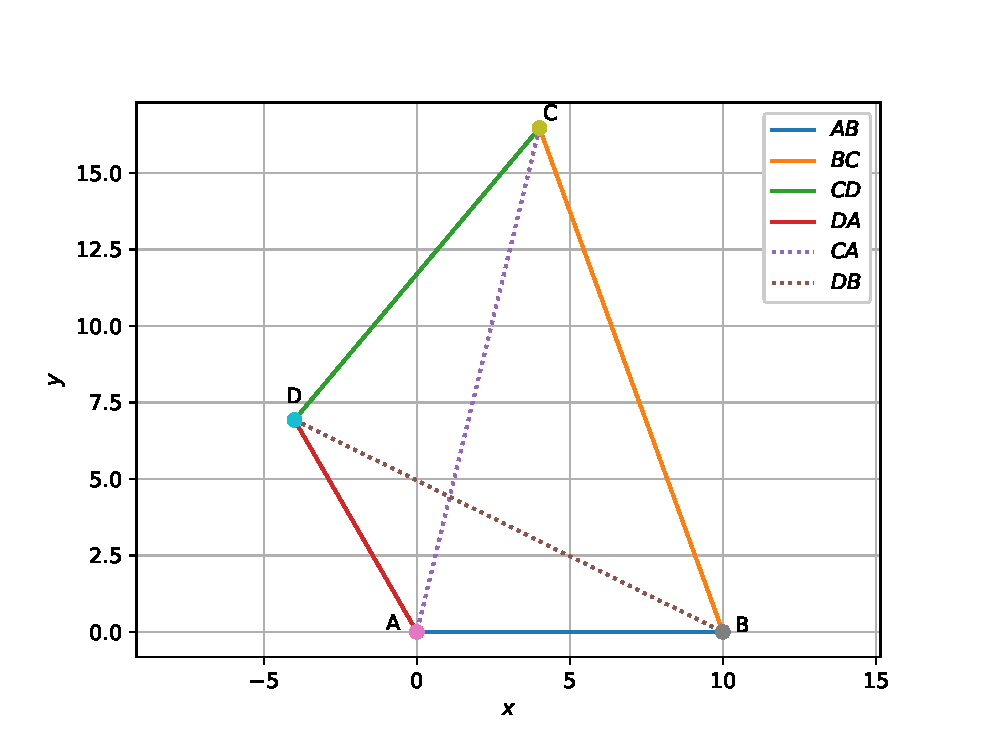
\includegraphics[width=\columnwidth]{./figs/quadilateral_ex/cyclic_quad.eps}
%\caption{Quadilateral generated using python}
%\label{fig:cyclic_quad2_quadilateral_ex}
%\end{figure} 
%
%The following Python code generates Fig. \ref{fig:cyclic_quad2_quadilateral_ex}
%
%\begin{lstlisting}
%codes/quadilateral_ex/cyclic_quad.py
%\end{lstlisting}
%\end{enumerate}
%\newpage
%
%
